\documentclass[aspectratio=169]{beamer}

\usetheme{Boadilla}
\setbeamersize{text margin left=12mm,text margin right=12mm}
\usepackage{biblatex} %Imports biblatex package
\addbibresource{adjointb.bib}

\usepackage{amsmath}
%\usepackage{txfonts}
\usepackage{amsfonts}
\usepackage{amssymb}
%\usepackage{calc}
\usepackage{graphicx}
\usepackage{graphbox}
\usepackage{breakurl}
\usepackage{xspace}
\usepackage{enumitem}
\usepackage{hyperref}
\usepackage{cleveref}	% must be loaded after hyperref
\usepackage[autostyle=true,german=quotes]{csquotes}
\usepackage{tikz-cd}
\usetikzlibrary{decorations.pathmorphing}
\usepackage[makeroom]{cancel}
\usepackage{mathabx}
\usepackage{multirow}
\usepackage{amssymb}
\usepackage{mathtools}
\usepackage{xfrac}
\usepackage{faktor}
\usepackage{stmaryrd}
%\usepackage[lite]{mtpro2}	% for super-wide tildes
% not found :/
\usepackage{tikzit}
\input{markov.tikzstyles}

% to strike out text:
\usepackage{ulem}
\renewcommand<>{\sout}[1]{
	\temporal#2{\invisible{#1}}{#1}{\beameroriginal{\sout}{#1}}
}

\title{An Introduction to Markov Categories}
%\subtitle{Paolo Perrone, IEEE Transactions on Information Theory, 2023}

\author[Utku, Nico, Drew]{Utku Boduroğlu, Drew McNeely, and Nico Wittrock}
\institute{Adjoint School 2024}
\date{April 11, 2024}

%some commands:
%cat stuff:
\newcommand{\cat}[1]{\mathsf{#1}}
\newcommand{\cC}{\cat{C}}
\DeclareMathOperator{\cop}{copy}
\DeclareMathOperator{\del}{del}
\newcommand{\idfun}	[1]{\operatorname{id}_{#1}}
\newcommand{\FinStoch}{\mathsf{FinStoch}}
\newcommand{\Stoch}{\mathsf{Stoch}}
\newcommand{\BorelStoch}{\mathsf{BorelStoch}}


\begin{document}

\begin{frame}
\titlepage
\end{frame}

\begin{frame}
	\frametitle{Outline}
	\tableofcontents
\end{frame}

%\section{Introduction to Markov Categories}
%%% Utku: Hey folks, I'm going to add comments here that I want to keep in context so that I can get your input and just discuss in-place instead of Zulip. 
% 
% I'm trying to lead the introduction part in the direction of the narrative
% that FinStoch and Stoch are the prototypical categories for the concept of a
% Markov category, and so the eventual definition of a Markov category that
% we'll reach is motivated by the inherent structure present in these two
% categories.
%
% Check my TODOs for my plans etc.
%

\subsection{Informal introduction to Markov kernels and Markov categories}

\begin{frame}
    A Markov category can be interpreted to consist of
    \begin{enumerate}\pause
        \item objects: spaces of possible values (Alphabets or data)\par
            Represented as wires\pause
            % TODO?: Add wire diagram
        \item morphisms: channels, devices, programs\par
            Represented as boxes, to be read horizontally from left to right

            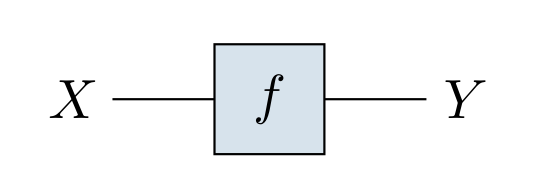
\includegraphics[width=.4\textwidth]{graphics/string/markov_morphism.png}
    \end{enumerate}\pause
    Morphisms are in general \emph{noisy}, involving randomness
\end{frame}

\begin{frame}
    \frametitle{Prototypical Markov categories}
    % Should this really be its own frame?
    \begin{enumerate}
        \item FinStoch: 
            \begin{itemize}
                \item objects: finite alphabets $X, Y, \dots$
                \item morphisms: stochastic matrices $f: X\to Y$
            \end{itemize}
        \item Stoch: 
            \begin{itemize}
                \item objects: measurable spaces/alphabets $(X, \Sigma_X), Y\ \text{(when clear from context)}, \dots$
                \item morphisms: Markov kernels $f: X\to Y$
            \end{itemize}
    \end{enumerate}
\end{frame}

\begin{frame}
    \frametitle{FinStoch}
    \framesubtitle{What are Stochastic matrices?}
    \begin{minipage}{.48\textwidth}
        A stochastic matrix from alphabet $X$ to alphabet $Y$ is a matrix of non-negative entries
        \begin{align*}
            X\times Y \to [0,1]\\
            (x, y) \mapsto f(y\mid x)
        \end{align*}
        such that each column sums to one:
        \[
            \sum_{y\in Y} f(y\mid x) = 1 \quad \text{for every $x\in X$.}
        \]
    \end{minipage}
    \hfill
    \begin{minipage}{.48\textwidth}
        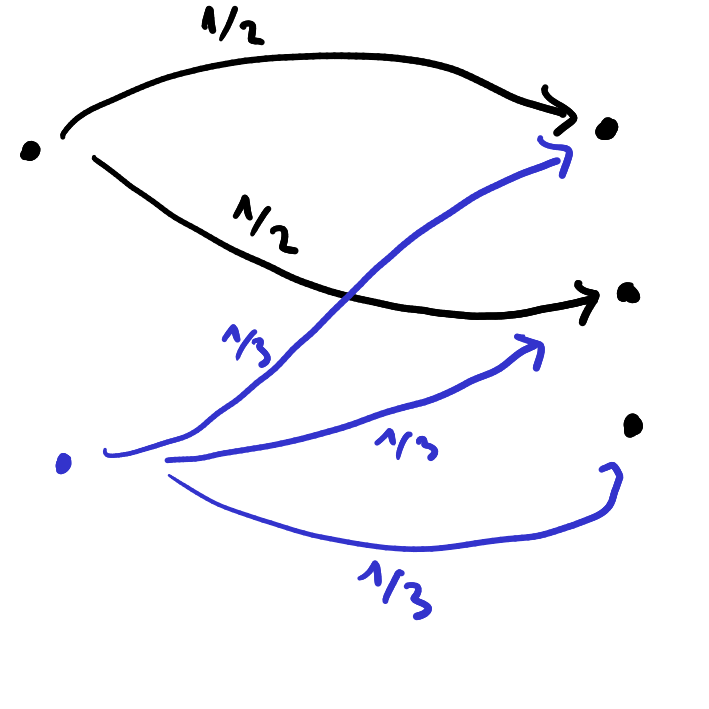
\includegraphics[width=\textwidth]{finstoch_mkv_kernel}
    \end{minipage}
\end{frame}

\begin{frame}
    \frametitle{Stoch}
    \framesubtitle{What are measurable spaces and Markov kernels?}
    % TODO?: do we talk about $\sigma$-algebras in detail
    A Markov kernel from measurable space $(X, \Sigma_X)$ to $(Y, \Sigma_Y)$ is an assignment
    \begin{align*}
        X\times \Sigma_Y \to [0, 1]\\
        (x, S) \mapsto f(S\mid x)
    \end{align*}
    which is measurable in $X$ and is a probability measure in $Y$.
\end{frame}

\begin{frame}
    For both examples, we can equivalently see the channels $X\to Y$ as (measurable) functions $X\to PY$, where for $x\in X$, $f_x$ is a probability measure of $Y$.\pause
    \[
        \text{\normalfont Hom} _\text{\normalfont Markov} (X, Y) \cong \text{\normalfont Meas} (X, PY)
    \]
    where $P$ is the probability (Giry) monad taking a measurable space $Y$ to the set (measurable space) of probability measures on $Y$.\pause

    \begin{minipage}{.3\textwidth}
        \begin{align*}
            X&\times Y \to [0, 1]\\
            X&\times \Sigma_Y \to [0, 1]\\
        \end{align*}
    \end{minipage}
    \hfill
    \begin{minipage}{.6\textwidth}
        \begin{align*}
            f_x: &Y\to [0, 1],\quad \sum\nolimits_{y\in Y} f(y \mid x) = 1\\
            f_x: &\Sigma_Y\to [0, 1] \in PY \\
        \end{align*}
    \end{minipage}
    % TODO: a short mention of probability monads here
    
\end{frame}

\subsection{Markov categories are categories}


\begin{frame}
    \frametitle{Composition}
    \framesubtitle{through the Chapman-Kolmogorov equation}
    % TODO: Shorten this frame
    % Composition (Stoch, FinStoch) through the Chapman-Kolmogorov equation (measure pushfwd, matmul)
    Given channels f : X → Y and g : Y → Z, we can form a channel g ◦ f : X → Z; for the case of Fin/Stoch, this is through the respective versions of the \emph{Chapman-Kolmogorov} formula:\pause
    \begin{itemize}
        \item in FinStoch,
        \begin{align}
            g\circ f (z\mid x) \coloneqq \sum_{y\in Y} g(z\mid y) f(y\mid x)
        \end{align}\pause
        \item in Stoch, it is given by the continuous analogue: for every measurable subset $S\subset Z$,
        \begin{align}
            g\circ f (S\mid x) \coloneqq \int_Y g(S\mid y) f(dy\mid x)
        \end{align}
        by which we mean the integral with respect to the measure $f_x$ on $Y$, for every $x$.
\end{itemize}
\end{frame}

\begin{frame}
    \frametitle{A basic example for $\mathsf{FinStoch}$}
    \begin{minipage}{.48\textwidth}
    The \emph{Chapman-Kolmogorov} formula:
    \begin{align*}
        g\circ f (z\mid x) \coloneqq \sum_{y\in Y} g(z\mid y) f(y\mid x)
    \end{align*}
    \end{minipage}
    \hfill
    \begin{minipage}{.45\textwidth}
        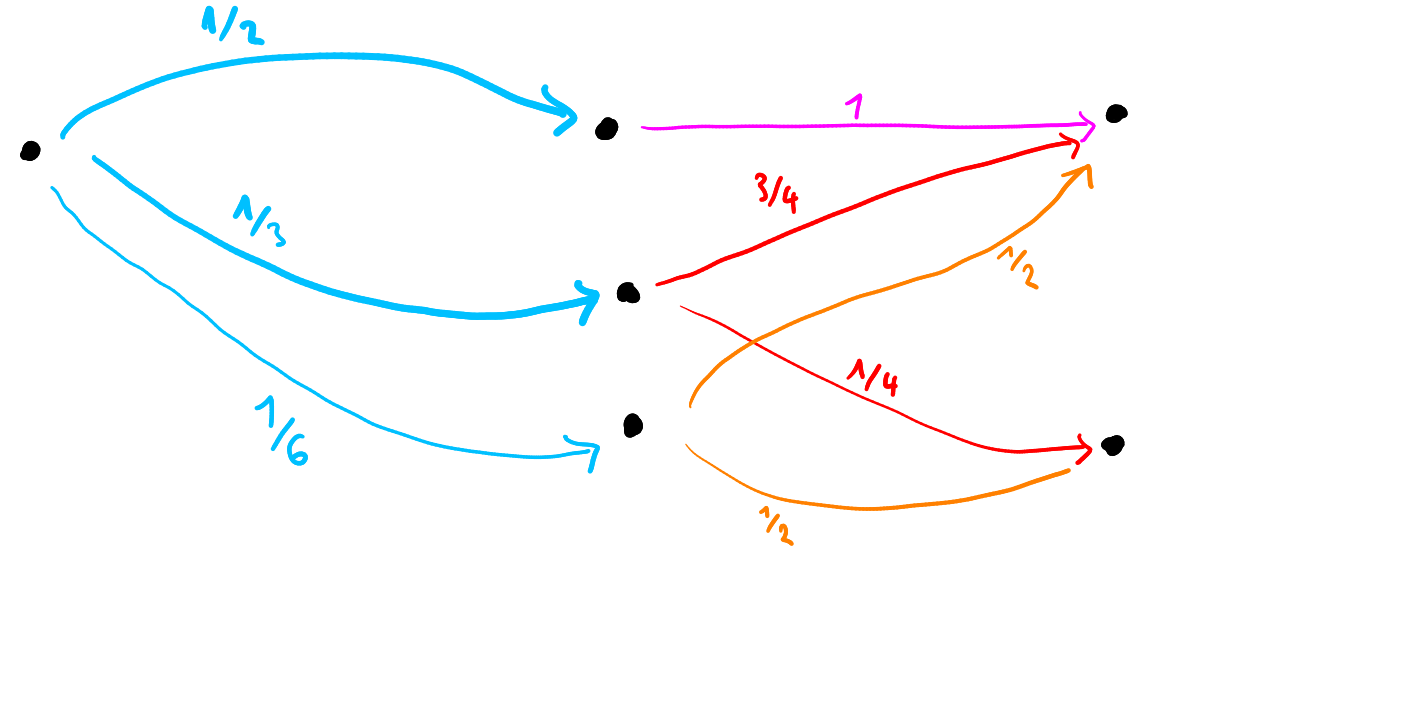
\includegraphics[width=\textwidth]{finstoch_matmul.png}
        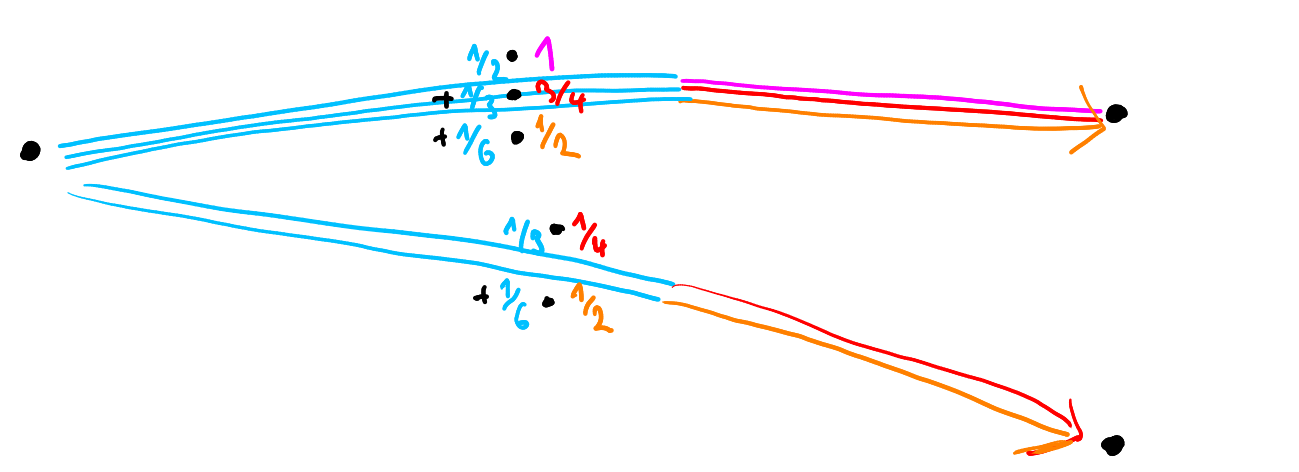
\includegraphics[width=\textwidth]{finstoch_matmul_2.png}
    \end{minipage}
    
\end{frame}

\begin{frame}
    \frametitle{Identity}
    \framesubtitle{through Dirac delta distribution}
    % TODO: Shorten this frame
    Identities in a Markov category represents for each object $X$ that there is no change in the state of $X$. We draw it simply with a wire.\pause
    \begin{itemize}
        \item In FinStoch, identities are identity matrices. 
        \item In Stoch, they are the "Dirac delta" kernels defined by the identity function
\end{itemize}
\begin{minipage}{.48\textwidth}
    \[
        \text{\normalfont id} (S\mid x) = \delta_x (S) = 1_S(x) = \begin{cases} 1\ x\in S\\ 0\ x\not \in S
        \end{cases}
    \]
\end{minipage}
\hfill
\begin{minipage}{.48\textwidth}
    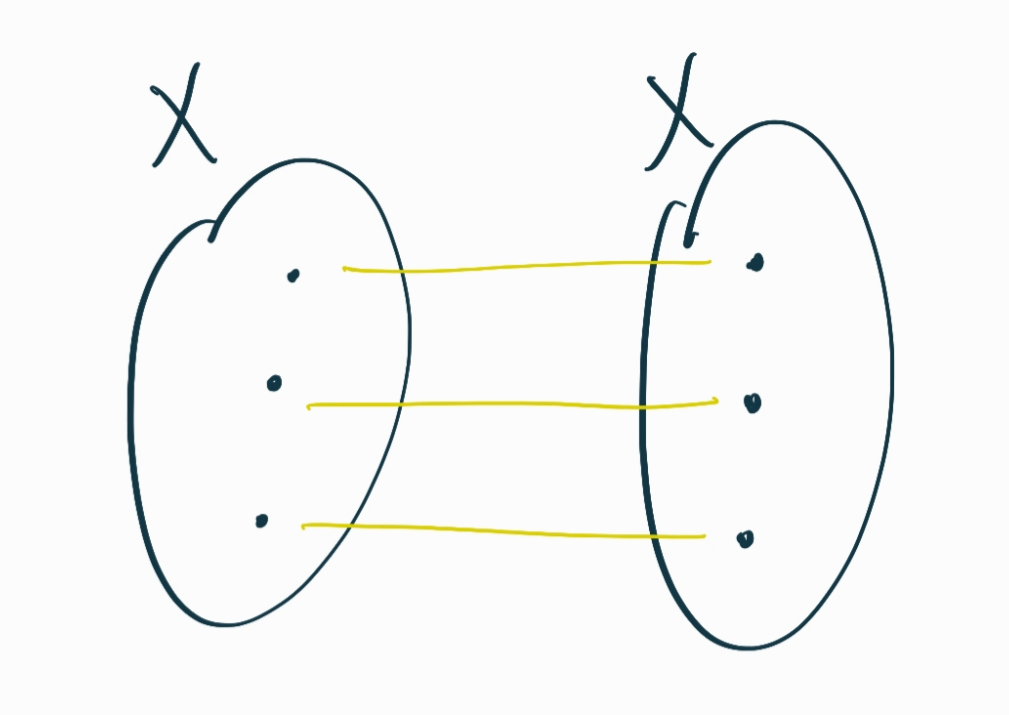
\includegraphics[width=\textwidth]{graphics/markov_delta.png}
\end{minipage}
\end{frame}


\subsection{Markov categories are symmetric monoidal}
\begin{frame}
    \frametitle{States}
    \framesubtitle{form probability distributions}
    % States form probability distributions
    % TODO: Rephrase to simplify what a source is in Fin/Stoch and what it should be in a MC
    Both $(\mathsf{FinStoch}, \otimes, *)$ and $(\mathsf{Stoch}, \otimes, *)$ are monoidal categories under "cartesian product" and the singleton space.\par
    In general, we have a unit, written $I$, and which we do not draw (it’s represented by an empty region).\pause

    \begin{minipage}{.55\textwidth}
        A source, or (random) state on X is now a morphism $p: I\to X$: 
    \end{minipage}
    \hfill
    \begin{minipage}{.4\textwidth}
        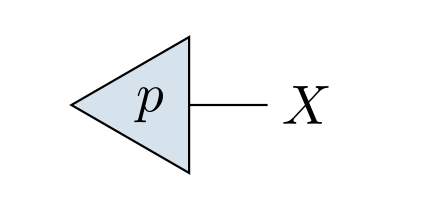
\includegraphics[width=\textwidth]{graphics/string/markov_state.png}
    \end{minipage}\pause

\begin{enumerate}
    \item FinStoch: a source is a stochastic "column" matrix, a finite probability measure on $X$
    \item Stoch: A Markov kernel to X with no input, i.e. a probability measure on $X$
\end{enumerate}

\end{frame}

\begin{frame}
    \frametitle{Parallel composition} 
Markov categories also come with a notion of parallel composition through $\otimes$\par
Given channels $f: X\to Y$ and $h: A\to B$, we can form the tensor product channel $f\otimes h: X\otimes A\to Y\otimes B$, which we represent as follows:\pause

\begin{minipage}{.4\textwidth}
    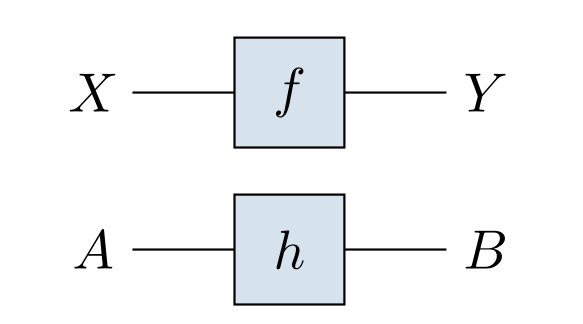
\includegraphics[width=\textwidth]{graphics/string/markov_parallel.png}
\end{minipage}
\hfill
\begin{minipage}{.55\textwidth}
    \[
        f\otimes h(y, b\mid x, a)\coloneqq f(y\mid x)h(b\mid a)
    \]
\end{minipage}
\end{frame}

\begin{frame}
    \begin{center}
        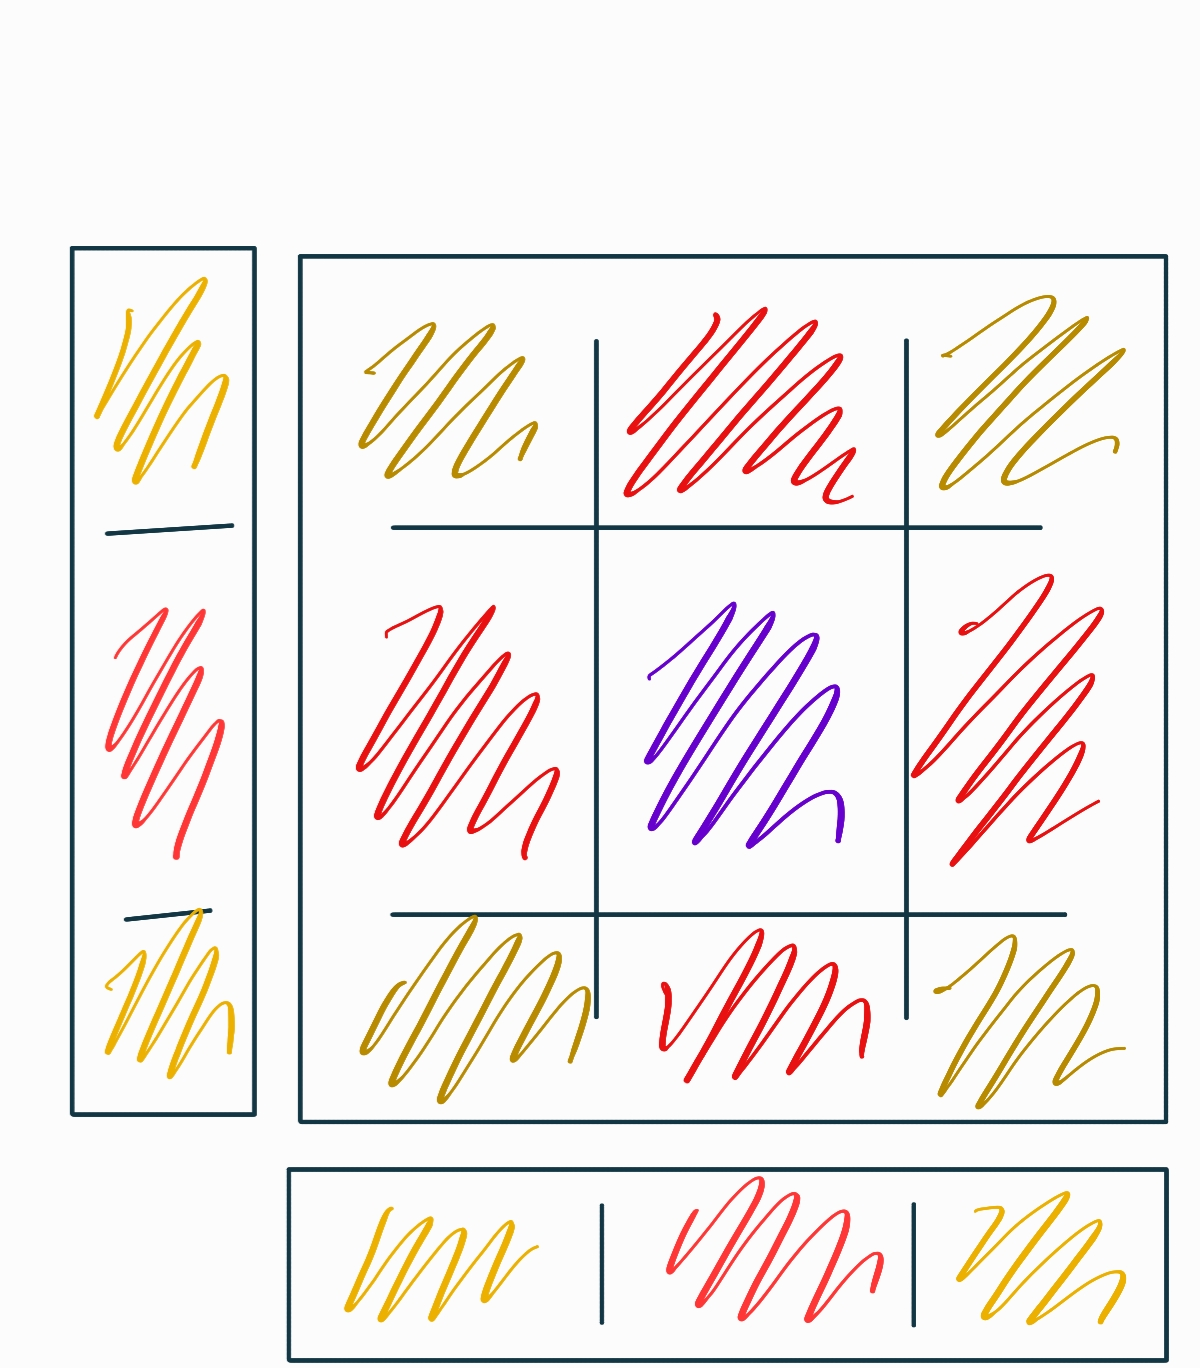
\includegraphics[width=.5\textwidth]{graphics/parallel_dist.jpg}
    \end{center}
\end{frame}

\subsection{Markov categories have comonoid objects}
\begin{frame}
    \frametitle{copy structure}
    \begin{minipage}{.57\textwidth}
        % The last piece of structure that we need to form a Markov category is two distinguished maps for each object X: a map $\text{\normalfont copy}: X\to X\otimes X$ which we call “copy” or “duplicate”, and represent as follows
        The copy structure consists of a copy (or duplicate) map ${\text{\normalfont copy} _X: X\to X\otimes X}$ for each object $X$, represented as

        \begin{center}
            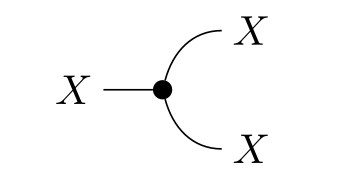
\includegraphics[width=.4\textwidth]{graphics/string/markov_copy.png}
        \end{center}

        As the name suggests, this can be thought of as making a copy of the information.
    \end{minipage}\pause
    \hfill
    \begin{minipage}{.38\textwidth}
        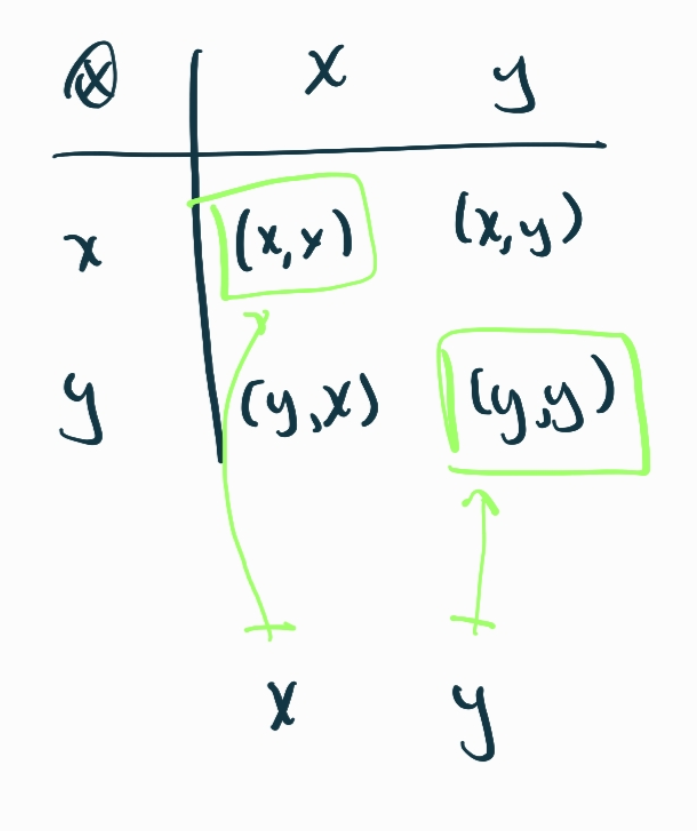
\includegraphics[width=\textwidth]{copy_illustration}
        % \caption{The grid above does NOT represent a stochastic matrix!}
    \end{minipage}
\end{frame}


\begin{frame}
    \frametitle{delete structure}
    The delete structure consists of a collection of maps
    \begin{minipage}{.48\textwidth}
        \[
            \text{\normalfont del} _X : X\to I
        \]
    \end{minipage}
    \hfill % 
    \begin{minipage}{.48\textwidth}
        \tikzfig{delete}
    \end{minipage}
    \vspace{5mm}

    for each object $X$. We also require that these morphisms assemble into a natural transformation $\text{\normalfont del} : \text{\normalfont id} \Rightarrow I$
\end{frame}

\begin{frame}[t]
    \frametitle{Marginals}
    \framesubtitle{with $\otimes$ and delete}
    \vspace{5mm}
    \begin{minipage}{.55\textwidth}
        With the compatible monoidal action and the delete structure, we can also talk about marginalization:\par
        For a joint morphism ${p: A\to X\otimes Y}$, we can obtain its marginal morphisms ${p|_X: A\to X}$ and ${p|_Y: A\to Y}$ by the delete map
        \begin{align*}
            (\text{\normalfont id} _X \otimes \text{\normalfont del} _Y) \circ p = p|_X\\
            (\text{\normalfont del} _X \otimes \text{\normalfont id} _Y) \circ p = p|_Y\\
        \end{align*}
    \end{minipage}
    \hfill
    \begin{minipage}{.35\textwidth}
        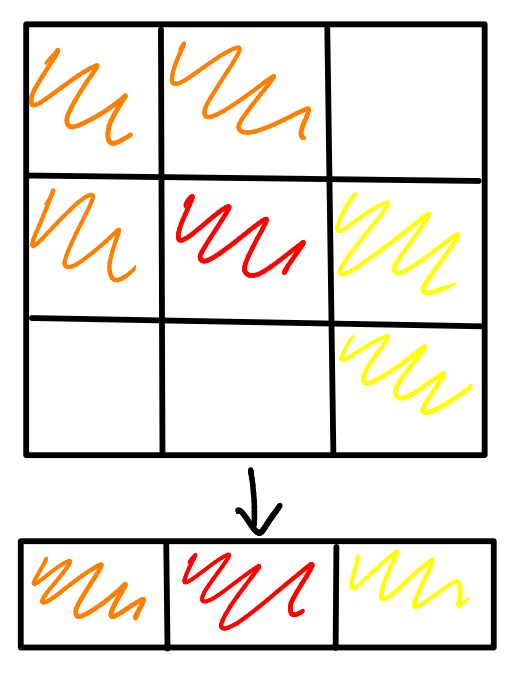
\includegraphics[width=\textwidth]{delete_graphic.png}
    \end{minipage}
\end{frame}

\begin{frame}[t]
    Graphically:
    \vspace{10mm}

    \begin{minipage}{.48\textwidth}
        \tikzfig{state_I}
    \end{minipage}
    \hfill
    \begin{minipage}{.48\textwidth}
        \tikzfig{marginalX_I}
    \end{minipage}
    \vspace{10mm}
    \pause

    \begin{minipage}{.48\textwidth}
        \tikzfig{state_A}
    \end{minipage}
    \hfill
    \begin{minipage}{.48\textwidth}
        \tikzfig{marginalX_A}
    \end{minipage}
\end{frame}

\begin{frame}
    \frametitle{Naturality of delete}
The last property that we require in a Markov category is normalization or counitality:

% applying a morphism f and discarding its output is the same as discarding the input from the start.  
% TODO: loop back to when we talked about normalization and say that naturality of delete suffices to reflect this
\begin{minipage}{.48\textwidth}
    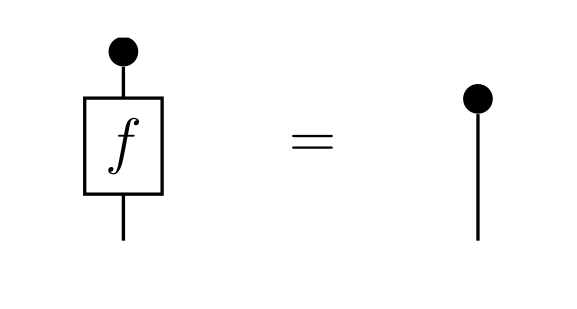
\includegraphics[width=\textwidth]{graphics/string/markov_nat_delete.png}
    % \tikzfig{normalization}
\end{minipage}
\hfill
\begin{minipage}{.48\textwidth}
% https://q.uiver.app/#q=WzAsMyxbMCwwLCJYIl0sWzIsMCwiSSJdLFswLDIsIlkiXSxbMiwxLCJcXHRleHR7ZGVsfV9ZIiwyXSxbMCwxLCJcXHRleHR7ZGVsfV9YIl0sWzAsMiwiZiIsMl1d
\[\begin{tikzcd}[ampersand replacement=\&]
	X \&\& I \\
	\\
	Y
	\arrow["{\text{del}_Y}"', from=3-1, to=1-3]
	\arrow["{\text{del}_X}", from=1-1, to=1-3]
	\arrow["f"', from=1-1, to=3-1]
\end{tikzcd}\]
\end{minipage}\pause

In FinStoch, this is exactly the condition that the sum of each column of a stochastic matrix is one, i.e. that transition probabilities are normalized.
\end{frame}

\subsection{Formal definition of Markov category}

\begin{frame}
    % “A Markov category is a semicartesian category where all objects are commutative comonoids compatible with the monoidal structure”
    \begin{definition}
        A Markov category is a symmetric monoidal category $(\mathsf{C}, \otimes, I)$ together with a chosen commutative comonoid structure for each object $X$, which is compatible with tensor products, and for which all morphisms are counital.
    \end{definition}\pause
    \begin{minipage}{.48\textwidth}
        \begin{enumerate}
            % minipages for each item??
            \item $\mathsf{C}$ is semi-cartesian
            \item Each object $X$ is equipped with "copy" and "discard" maps
            \item which satisfy the identities of a commutative monoid
            \item The copy maps are compatible with the monoidal structure in the following way
        \end{enumerate}
    \end{minipage}
    \hfill
    \begin{minipage}{.48\textwidth}
        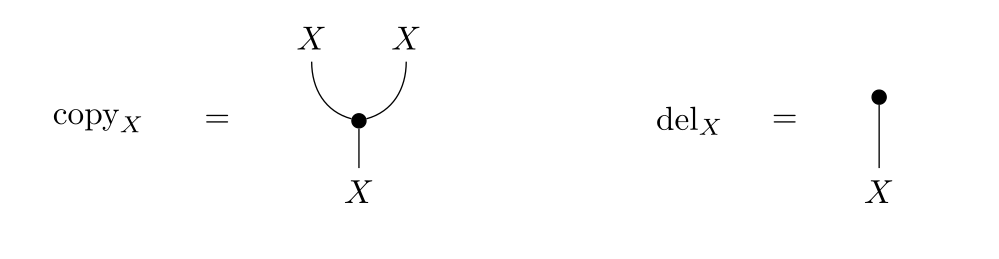
\includegraphics[width=\textwidth]{graphics/string/markov_copy_delete.png}
        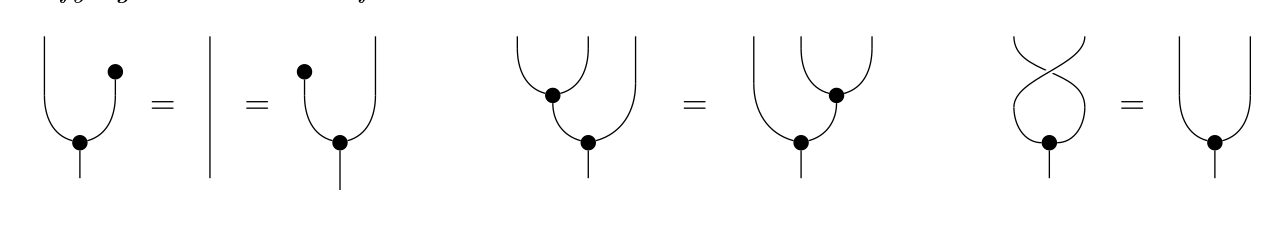
\includegraphics[width=\textwidth]{graphics/string/markov_commutative_monoid.png}
        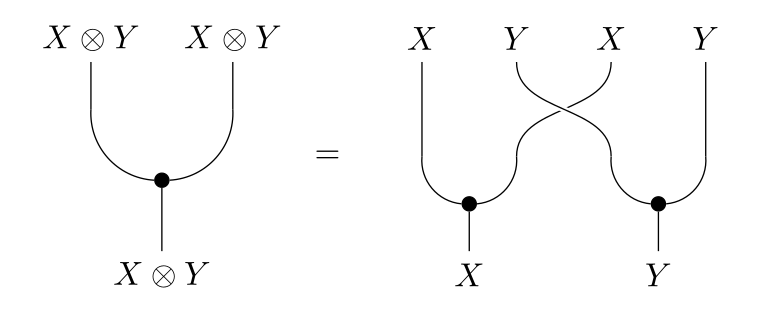
\includegraphics[width=\textwidth]{graphics/string/markov_monoidal_compat.png}
    \end{minipage}
\end{frame}

%\section{Uncertainty in Markov categories}
%\begin{frame}
	This is part 2... so far
\end{frame}
\section{Properties and additional axioms}
\begin{frame}{Independence of states}
\tikzfig{state-independence}
\end{frame}

\begin{frame}{Independence conditioned on an input}
\tikzfig{input-independence}
\end{frame}

\begin{frame}{Independence conditioned on an output}
\tikzfig{output-independence}
\end{frame}

\begin{frame}{Independence conditioned on combined input and output}
\tikzfig{combined-independence}
\end{frame}

\begin{frame}{Conditionals}
\tikzfig{conditional}
\end{frame}

\begin{frame}{Correlation}
\tikzfig{conditional-independent}
\end{frame}

\begin{frame}{Almost Sure Equality}
\tikzfig{almost-surely}
\end{frame}

\begin{frame}{Uniqueness of conditionals}
\tikzfig{conditional-uniqueness}
\end{frame}

\begin{frame}{Dashed Box Notation}
\tikzfig{dashed-box-notation}
\end{frame}

\begin{frame}{Rewrite Rules}
\tikzfig{conditional-rewrites}
\end{frame}

\begin{frame}{Bayesian Inversion}
\tikzfig{bayesian-inverse}
\end{frame}


\begin{frame}{Literature}
\printbibliography
\end{frame}

\begin{frame}
	Questions
\end{frame}

\section{Bonus Slides}
\subsection{Powerset monad}

\begin{frame}{Probability Monads}
	\begin{example}[Powerset Monad]
		$\cat{Set}$ is cartesian monoidal $\Rightarrow$ morphisms are deterministic
		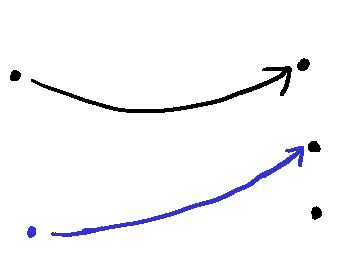
\includegraphics[scale=0.4]{part2/Figures/morphisms_set}
%		\pause 
		\begin{equation*}
		\begin{split}
		\text{Powerset monad} ~
		2^{\bullet} : \cat{Set} &\to \cat{Set}, \quad \\
		X &\mapsto 2^X := \{ M \subseteq X \}
		\end{split}
		\end{equation*}
%		\pause
		\begin{minipage}{0.69\linewidth}
			Kleisli category $\cat{Set}_{2^{\bullet}}$ has morphisms: 
			\begin{equation*}
			\begin{split}
				f : X &\to 2^Y	
				\quad \text{i.e.~}
				f(x) \subseteq Y
			\end{split}
			\end{equation*}
			As Pablo stated: describes \emph{possibility}
	\end{minipage}
	\begin{minipage}{0.3\linewidth}
		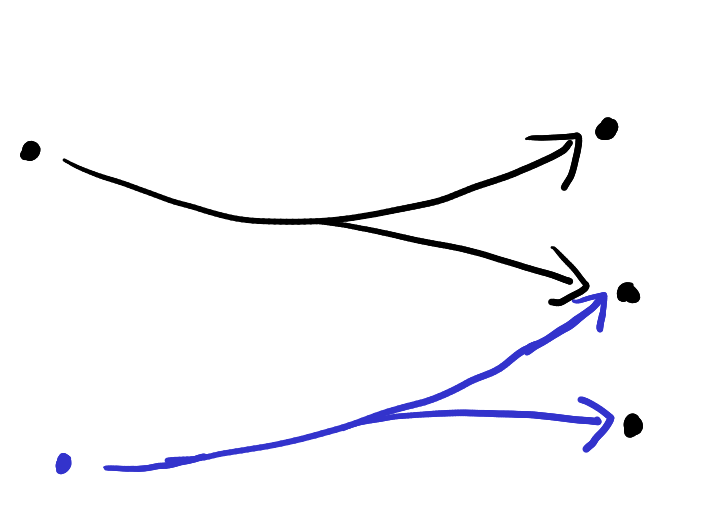
\includegraphics[scale=0.4]{part2/Figures/morphisms_poss}
	\end{minipage}
%	Problem: \enquote{impossibility}
%	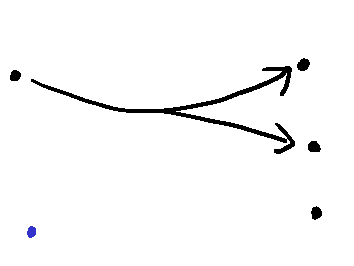
\includegraphics[scale=0.4]{part2/Figures/morphisms_no_poss}
	\end{example}
\end{frame}

\begin{frame}{Probability Monads}
	\begin{example}[Powerset Monad]
%		$\cat{Set}$ is cartesian monoidal $\Rightarrow$ morphisms are deterministic
%		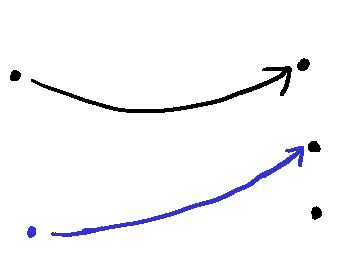
\includegraphics[scale=0.4]{part2/Figures/morphisms_set}
%%		\pause 
%		\begin{equation*}
%		\begin{split}
%		\text{Powerset monad} ~
%		2^{\bullet} : \cat{Set} &\to \cat{Set}, \quad \\
%		X &\mapsto 2^X := \{ M \subseteq X \}
%		\end{split}
%		\end{equation*}
%%		\pause
		\begin{minipage}{0.74\linewidth}
			Problem: Kleisli category $\cat{Set}_{2^{\bullet}}$ has morphism: 
			\begin{equation*}
			\begin{split}
			f : X &\to 2^Y	
			\quad \text{with} \quad
			f(x_i) = \emptyset
			\end{split}
			\end{equation*}
%			this describes \emph{im}possibility
		\end{minipage}
		\begin{minipage}{0.25\linewidth}
			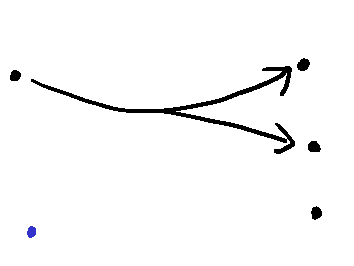
\includegraphics[scale=0.4]{part2/Figures/morphisms_no_poss}
		\end{minipage}
		\pause
		\begin{equation*}
			\tikzfig{counitality_l}
			= 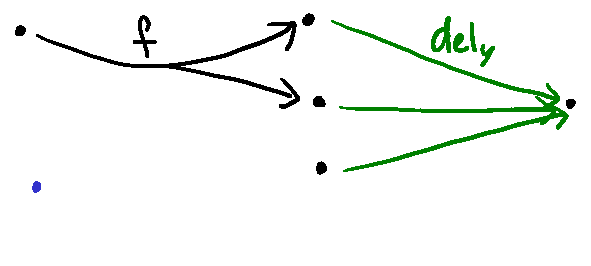
\includegraphics[scale=0.3]{part2/Figures/morphisms_no_poss_composed_1}
			= 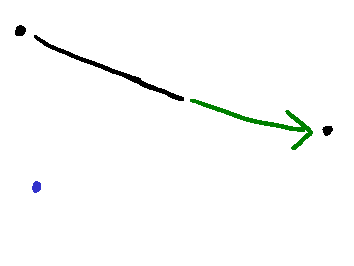
\includegraphics[scale=0.3]{part2/Figures/morphisms_no_poss_composed_2}
			\neq 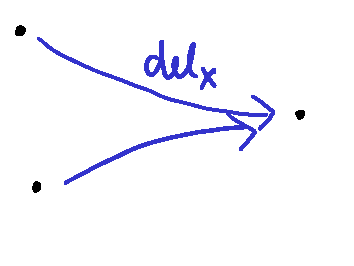
\includegraphics[scale=0.3]{part2/Figures/morphisms_no_poss_composed_3}
			= \tikzfig{counitality_r}
		\end{equation*}
%		\pause
		$\Rightarrow$ $\cat{Set}_{2^{\bullet}}$ is \emph{not} Markov! 
%		\pause
%		\\ $\rightsquigarrow$ adjust monad:
		\begin{equation*}
		\begin{split}
				\rightsquigarrow \text{adjust monad} \quad
				T : \cat{Set} &\to \cat{Set}, \quad \\
				X &\mapsto 2^X - \emptyset
		\end{split}
		\end{equation*}
%		\pause
		$\Rightarrow$ $\cat{Set}_{T} =: \cat{Poss}$ is Markov. \pause With uncertainty.
	\end{example}
\end{frame}

%\section{Markov Categories}
%\subsection{Axioms}
%
%\begin{frame}
%\frametitle{Definition of Markov Category}
%\begin{definition}
%	A Markov category is a semi-Cartesian category in which every object is a commutative comonoid.
%\end{definition}
%\end{frame}
%
%\subsection{Examples}
%
%\begin{frame}
%	\frametitle{Example Markov category}
%	Okay if we create an example, it absolutely needs to involve the cloud cover forecast during the total solar eclipse.
%\end{frame}
%
%\section{Enriched Categories}
%
%\begin{frame}
%	\frametitle{Enriched Categories}
%	So yeah an enriched category is like a category with more structure on the morphisms.
%	Instead of having hom-sets, ya got yourself some hom-objects.
%\end{frame}
%
%\section{Divergences}
%
%\begin{frame}
%	\frametitle{Divergence}
%	Aight, so a divergence is like a metric for probability distributions...
%
%	Except it ain't a metric, cause it ain't \emph{sym}metric.
%\end{frame}
%
%\subsection{Entropy}
%
%\begin{frame}
%	\frametitle{Entropy}
%	Entropy is a measure of how ``random'' a probability distribution is, given through the divergence between both sides of the defining equation for deterministic kernels. Neat!!
%\end{frame}

\end{document}
